\documentclass{ecai2012}
\usepackage{times}
\usepackage{enumerate}
\usepackage{algpseudocode}
\usepackage[ruled]{algorithm}
\usepackage{url}
\usepackage{framed}
\usepackage{amsfonts,amsmath,amsthm,amssymb}
\usepackage{graphicx}
\usepackage{url}
\usepackage{color}
\usepackage{geometry}

\geometry{margin=1.2in}

\newcommand {\mean} {\ensuremath {\mathop{\mathrm{mean}}}}
\newcommand {\median} {\ensuremath {\mathop{\mathrm{median}}}}
\newcommand {\N} {\ensuremath {\mathcal{N}}}
\newcommand {\IE} {\ensuremath {\mathbb{E}}}
\newcommand {\cov} {\ensuremath {\mathop{\mathrm{cov}}}}
\newcommand {\BEL} {\ensuremath {\mathop{\mathrm{BEL}}}}

\newtheorem{dfn}{Definition}
\newtheorem{thm}{Theorem}
\newtheorem{lmm}{Lemma}
\newtheorem{crl}{Corollary}

\title{VOI-aware MCTS}
%\author {David Tolpin, Solomon Eyal Shimony \\
%Department of Computer Science, \\
%Ben-Gurion University of the Negev, Beer Sheva, Israel \\
%\{tolpin,shimony\}@cs.bgu.ac.il}

\begin{document}

\maketitle

\begin{abstract}
Upper bounds for the VOI are provided for pure exploration in the
MCTS. A sampling policy based on the upper bounds is
suggested. Empirical evaluation of the policy and comparison to UCB1
and UCT is performed on random bandit instances as well as on Computer
Go.
\end{abstract}


\section{Introduction and Definitions}

Taking a sequence of samples in order to minimize the
regret of a decision based on the samples is abstracted by the
{\em Multi-armed Bandit Problem.} In the Multi-armed Bandit problem
we have a set of $K$ arms. Each arm can be pulled multiple
times. When the $i$th arm is pulled, a random reward $X_i$ from an
unknown stationary distribution is returned.  The reward is bounded
between 0 and 1.

The simple regret of a sampling policy for the Multi-armed Bandit
Problem is the expected difference between the best expected reward
$\max\limits_i\IE[X_i]$ and the expected reward $\IE[X_j]$ of the arm
with the best sample mean $\overline X_j=\max\limits_i\overline X_i$:
\begin{equation}
\label{eqn:simple-regret}
\IE[R]=\sum_{j=1}^K\Delta_j\Pr(\overline X_j=\max_i\overline X_i)
\end{equation}
where $\Delta_j=\max\limits_i\IE[X_i]-\IE[X_j]$.  Strategies that
minimize the simple regret are called pure exploration strategies
\cite{Bubeck.pure}. Principles of rational metareasoning
\cite{Russell.right} suggest that at each step the arm with the
greatest value of information (VOI) estimate must be pulled, and the
sampling must be stopped and a decision must be made when no arm has
positive VOI estimate.

In order to estimate the VOI of pulling an arm, a sampling model is
needed.  The generic sampling model used is: 
\begin{itemize}
\item The actual value of an arm has a certain distribution.
\item Pulling an arm is an i.i.d. noisy measurement of the actual
  value of the arm.
\end{itemize}
In \cite{HayRussell.MCTS}, Section 4, two instances of this model are
examined:
\begin{enumerate}[a)]
\item uniformly distributed prior of the value, with Bernouli
  sampling, and 
\item normally distributed prior of the value, with normally
  distributed sampling.
\end{enumerate}
Here we examine the same general setting (i.i.d. samples), but instead
of using a specific distribution model, use {\em concentration
inequalities} to derive distribution-independent bounds on the
VOI. Our bounds are applicable to any bounded distribution. Similar
bounds can be derived for certain unbounded distributions, such as the
normally distributed prior of the value with normally disributed
sampling, a subject of future work.

\section{Related Work}

Efficient algorithms for Multi-Armed Bandits based on
distribution-independent bounds, in particular UCB1, are introduced in
\cite{Auer.ucb}. The UCT algorithm, an extension of UCB1 to
Monte-Carlo Tree Search is described in \cite{Kocsis.uct}, and a successful
application of UCT to playing the Go game is discussed in
\cite{Gelly.mogo}.

Pure exploration in Multi-armed bandits is explored in
\cite{Bubeck.pure}. On the one hand, the paper proves certain upper
and lower bounds for UCB1 and uniform sampling, showing that an upper
bound on the simple regret is exponential in the number of samples for
uniform sampling, while only polynomial for UCB1. On the other hand,
empirical performance of UCB1 appears to be better than of uniform
sampling. \cite{Mnih.bernstop} investigate stopping criteria for
sampling based on the empirical Bernstein inequality; however, the
stopping criteria are based on error probabilities rather than on
value of information measures, and do not directly address the
objective of regret minimization.

The principles of bounded rationality appear in
\cite{Horvitz.reasoningabout}. \cite{Russell.right} provided a formal
description of rational metareasoning and case studies of applications
in several problem domains. One obstacle to straightforward
application of the principles of rational metareasoning to Monte-Carlo
sampling is the metagreedy assumption, according to which samples must
be selected as though at most one sample can be taken before an action
is chosen. In Monte-Carlo sampling, the value of information of any
single sample in a given search state is often zero, so a different
approximating assumption must be used instead.

\section{Upper Bounds on Value of Information}

The intrinsic VOI $\Lambda_i$ of pulling an arm is the expected decrease
in the regret compared to selecting an arm without pulling any arm at
all. Two cases are possible:
\begin{itemize}
\item the arm $\alpha$ with the highest sample mean is pulled, and the 
actual arm value is lower than the sample mean of the second-best arm $\beta$;
\item another arm is pulled, and the actual arm value is higher
than the sample mean of the best arm $\alpha$.
\end{itemize}
The \textit{myopic} VOI estimate is of limited applicability to
Monte-Carlo sampling, since the effect of a single sample is small,
and the myopic VOI estimate will often be zero, resulting in premature
termination of the search. However, $\Lambda_i$ can be estimated as the intrinsic 
value of information $\Lambda_i^b$ of pulling the $i$th arm for the
rest of the budget of $N$ samples:
\begin{thm} Denote the current number of samples of the $i$th arm by
  $n_i$. $\Lambda_i^b$ is bounded from above as
\begin{equation}
  \Lambda_i^b \le \left\{
  \begin{array}{l l}
    \overline X_\beta\frac N {N+n_i}\Pr(\overline X_i'\le\overline X_\beta)
    \le N\frac {\overline X_\beta} {n_i}\Pr(\overline X_i'\le\overline X_\beta) & \mbox{{\rm if} $i=\alpha$} \\
    (1-\overline  X_\alpha)\frac N {N+n_i}\Pr(\overline X_i'\ge\overline X_\alpha)
       \le N\frac {(1-\overline  X_\alpha)} {n_i}\Pr(\overline X_i'\ge\overline X_\alpha) & \mbox{\rm otherwise}
  \end{array} \right.
\label{eqn:thm-be}
\end{equation}
where $\overline X_i'$ is the sample mean of the $i$th arm after $n_i+N$ samples.
\label{thm:be}
\end{thm}

The probabilities can be bounded from above using the
Hoeffding inequality \cite{Hoeffding.ineq}.
\begin{thm} The probabilities in equations (\ref{eqn:thm-be}) are bounded from above as
\begin{align}
\Pr&(\overline X_\alpha' \le \overline X_\beta)
  \le 2\exp\left(- \varphi(n_\alpha)(\overline X_\alpha - \overline X_\beta)^2 n_\alpha
   \right)\nonumber\\
\Pr&(\overline X_i' \ge \overline X_\beta)
   \le 2\exp\left(- \varphi(n_i) (\overline X_\alpha -\overline  X_i)^2 n_i \right)
\label{eqn:probound-blnk-hoeffding}
\end{align}
where $\varphi(n)=2(\frac {1+n/N} {1+\sqrt {n/N}})^2 \ge 1.37$.
\label{thm:hoeffding-prob-bounds}
\end{thm}

\begin{crl}
An upper bound on the VOI estimate $\Lambda_i^b$ is obtained
by substituting (\ref{eqn:probound-blnk-hoeffding}) into (\ref{eqn:thm-be}).
\begin{equation}
  \Lambda_i^b \le \hat\Lambda_i^b=\left\{
  \begin{array}{l l}
    N\frac {\overline X_\beta} {n_i}\cdot 2\exp\left(- 1.37(\overline X_i - \overline X_\beta)^2 n_i\right)
      & \mbox{{\rm if} $i=\alpha$} \\
    N\frac {(1-\overline  X_\alpha)} {n_i}\cdot 2\exp\left(- 1.37(\overline X_\alpha - \overline X_i)^2 n_i\right)
      &  \mbox{\rm otherwise}
  \end{array} \right.
\label{eqn:bound-blnk-hoeffding}
\end{equation}
\label{crl:bound-blnk-hoeffding}
\end{crl}
Estimate $\hat\Lambda_i^b$ can be viewed as a
relaxation of the myopic assumption such that sequences consisting
of more than one action are taken into considertion.

\section{VOI-based Sample Allocation}

Following the principles of rational metareasoning, an arm with
the highest VOI should be pulled at each step. The upper bounds
established in Corollary~\ref{crl:bound-blnk-hoeffding} can be used
as VOI estimates. As illustrated by the empirical evaluation
(Section~\ref{sec:empirical-evaluation}), estimates based on upper
bounds on the VOI result in rational sampling policies, and exhibit
performance comparable to the performance of some state-of-the-art
heuristic algorithms.

\section{Empirical Evaluation}
\label{sec:empirical-evaluation}

\subsection{Selecting The Best Arm}
\label{sec:emp-arm}

\begin{figure}[t]
\centering
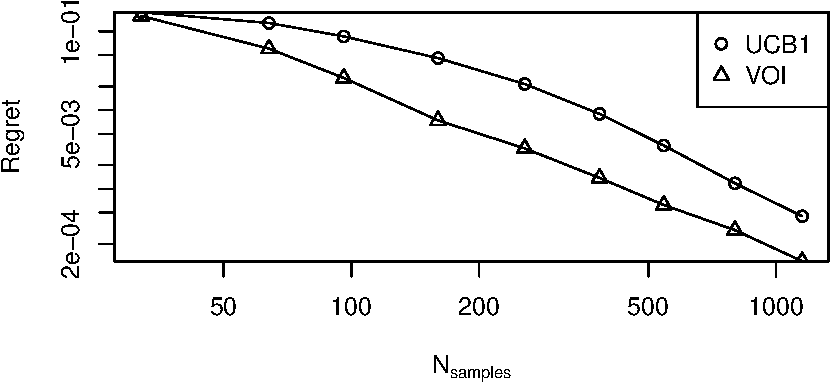
\includegraphics[scale=0.5]{flat.pdf}
\caption{Random instances: regret vs. number of samples}
\label{fig:random-instances}
\end{figure}

The sampling policies are first compared on random Multi-armed bandit 
problem instances. Figure~\ref{fig:random-instances} shows results for
randomly-generated Multi-armed bandits with 32 Bernoulli arms, with
the mean rewards of the arms distributed uniformly in the range $[0,
  1]$, for a range of sample budgets $32..1024$, with multiplicative
step of $2$. The experiment for each number of samples was repeated
10000 times. UCB1 is always considerably worse than the
VOI-aware sampling policy.

\subsection{Playing Go Against UCT}
\label{sec:emp-go}

The policies were also compared on Computer Go, a  search domain
in which UCT-based MCTS has been particularly successful
\cite{Gelly.mogo}. A modified version of Pachi \cite{Braudis.pachi}, a state of the art
Go program, was used for the experiments. The UCT engine was extended
with a VOI-aware sampling policy, and a time allocation mode ensuring
that both the original UCT policy and the VOI-aware policy use the
same average number of samples per node was added. (While the UCT
engine is not the most powerful engine of Pachi, it is still a strong
player; on the other hand, additional features of more advanced
engines would obstruct the MCTS phenomena which are the subject of
the experiment.)
\begin{figure}[t]
\centering
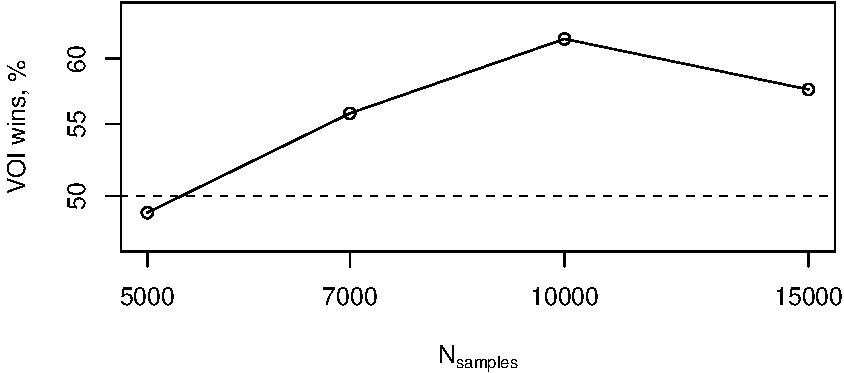
\includegraphics[scale=0.5]{vct-wins.pdf}
\caption{Go: winning rate --- UCT against VCT}
\label{fig:vct-against-uct}
\end{figure}
The engines were compared on the 9x9 board, for 5000, 7000, 1000, and
15000 samples per ply, each experiment was repeated
1000 times. Figure~\ref{fig:vct-against-uct}
shows the winning rate of VOI+UCT against UCT vs. the number of
samples. For most numbers of samples per node, VOI+UCT outperforms UCT.

\section{Summary and Future Work}

This work suggested Monte-Carlo sampling policies in which sample
selection and termination are based on upper bounds on the value of
information. A simplified model of accounting for future value of
information of a sample, based on early termination and sample
redistribution, was proposed for Monte-Carlo sampling in
trees. Empirical evaluation showed that these policies outperform
heuristic algorithms for simple regret minimization in Multi-armed
bandits, as well as for tree search.

Monte-Carlo tree search still remains a largely unexplored field of
application of VOI-aware algorithms. More elaborated VOI estimates,
taking into consideration re-use of samples in future search states
should be considered. The policies introduced in the paper differ from
the UCT algorithm only at the first step, where the VOI-aware
decisions are made. Consistent application of principles of rational
metareasoning at all steps of a rollout may further improve the
sampling policies.


\bibliographystyle{ecai2012}
\bibliography{refs}

\end{document}
